\chapter{Визуалицаия с помощью Python}
\label{ch:chap3}

Сложим 2 сигнала с одинаковой частотой, но разными фазами и амплитудой. Получим новый сигнал с новой амплитудой и новой фазой

\begin{figure}[ht]
    \centering
    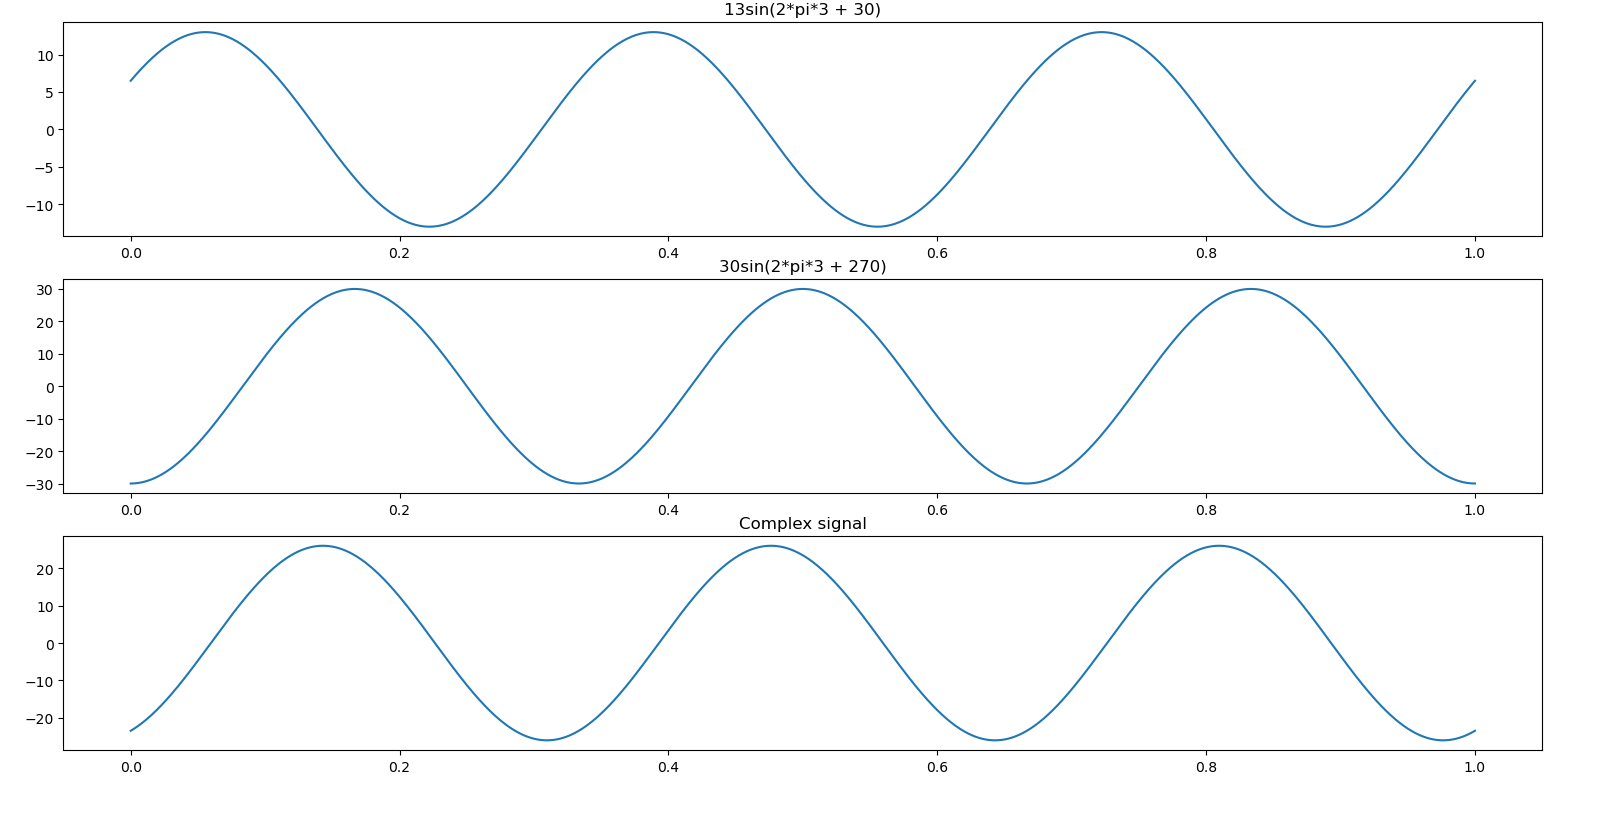
\includegraphics[width=1.0\textwidth]{same_freq.png}
    \caption{Результат сложения сигналов с совпадающей частотой}
\end{figure}

\endinput